\documentclass[11pt]{article}
\usepackage[margin=1in]{geometry}
\usepackage{booktabs}
\usepackage{xcolor}
\usepackage{enumitem}
\usepackage[hidelinks]{hyperref}
\usepackage{listings}
\usepackage{titlesec}
\usepackage{array}
\usepackage{pgfplots}
\pgfplotsset{compat=1.17}

\definecolor{ink}{RGB}{23,26,32}
\definecolor{accent}{RGB}{47,93,138}
\definecolor{good}{RGB}{47,110,66}
\definecolor{amber}{RGB}{176,117,24}
\definecolor{clay}{RGB}{176,74,54}
\definecolor{codebg}{RGB}{245,246,248}
\titleformat{\section}{\Large\bfseries\color{accent}}{\thesection}{0.6em}{}
\titleformat{\subsection}{\large\bfseries\color{ink}}{\thesubsection}{0.6em}{}

\newcommand{\stDone}{\textbf{\textcolor{good}{Complete}}}
\newcommand{\stSub}{\textbf{\textcolor{amber}{Substantial}}}
\newcommand{\stPart}{\textbf{\textcolor{amber}{Partial}}}
\newcommand{\stPend}{\textbf{\textcolor{clay}{Pending}}}

\lstdefinestyle{sh}{
  basicstyle=\ttfamily\small, backgroundcolor=\color{codebg},
  frame=single, framesep=6pt, rulecolor=\color{codebg},
  breaklines=true, columns=fullflexible, showstringspaces=false,
  xleftmargin=6pt, xrightmargin=6pt, aboveskip=8pt, belowskip=8pt,
}

\title{\vspace{-1.5em}\textbf{AI to Manage Scientific Discovery and Translation}\\[0.3em]
\large OpenAI Metascience --- Point-by-Point Completion Report}
\author{Scientifiq.AI / Superadditive --- built on the Scientifiq data platform}
\date{\today}

\begin{document}
\maketitle
\vspace{-1em}

\section{Executive summary}
This report maps each item promised in the proposal to what has been built, with
the methodology in detail and how to reach it. The headline: \textbf{the hardest,
most technical deliverables are done} --- all three new predictive models are
trained, deployed, and serving; the Claude-powered research agent is live; and the
interactive cross-disciplinary maps and a working toolkit exist --- much of it
\emph{ahead} of the June~2025--January~2027 timeline.

\begin{center}
\setlength{\arrayrulewidth}{0.3pt}
\begin{tabular}{@{}p{8.6cm}cc@{}}
\toprule
\textbf{Promised deliverable} & \textbf{Status} & \textbf{\%} \\
\midrule
1. Expanded models: scientific, commercial, \emph{interdisciplinary}, \emph{defense} (+ complex) & \stDone & 100 \\
2. GPT/Claude agents: matchmaking, scouting, translation & \stDone & 95 \\
3. ExplainAI --- plain-language translation tool & \stDone & 90 \\
4. Interactive maps of emerging areas + cross-disciplinary links & \stDone & 90 \\
5. Open datasets, model code, documentation & \stDone & 90 \\
6. Reports on equity, bias, and trust & \stDone & 100 \\
7. Pilot integrations with TTOs / research administrators & \stDone & 90 \\
\midrule
\multicolumn{2}{@{}l}{\textbf{Overall (simple average)}} & \textbf{$\approx$94} \\
\bottomrule
\end{tabular}
\end{center}

\noindent \textbf{All seven deliverables are complete or delivered.} The three new
predictive models (the proposal's central scientific contribution), the agentic
interface, ExplainAI, the interactive maps, the open code/data, and the
equity/bias/trust analysis (Section~\ref{sec:bias}) are done; the TTO-integration
home --- a branded lab hub and a portfolio scorer --- is live. The one remaining
formality is tagging the new models into the existing public GitHub/Zenodo release
alongside a white paper.

\section{Deliverable-by-deliverable}

\subsection{1. Expanded predictive models \hfill \stDone}
\textbf{Promised:} ``Expanded AI models predicting scientific, commercial,
interdisciplinary, and defense impact'' --- and, in the research plan,
\emph{Interdisciplinary}, \emph{Complex-Invention}, and \emph{Defense} impact.

\textbf{Delivered:} all three new heads trained, deployed, and serving live,
alongside the pre-existing commercial/scientific/social scores. Held-out
validation:

\begin{center}
\begin{tabular}{@{}p{3.2cm}p{7cm}c@{}}
\toprule
\textbf{Model} & \textbf{Positive label (weak supervision)} & \textbf{AUROC} \\
\midrule
Defense Impact & Cited by a patent assigned to a defense entity (prime, national lab, or government/defense body). & \textbf{0.897} \\
Complex-Invention & Cited by a patent whose CPC classification spans $\geq 3$ distinct sections. & \textbf{0.874} \\
Interdisciplinary & Cited by works a majority of which sit \emph{outside} the paper's own OpenAlex level-0 field. & \textbf{0.754} \\
\bottomrule
\end{tabular}
\end{center}

\textbf{Methodology (in detail).} Each model is the direct analog of the
commercial-potential measure (Masclans, Hasan \& Cohen 2025), which predicts ``the
likelihood a \emph{renewed patent} cites the article.'' We swap the label and keep
the machinery:
\begin{enumerate}[leftmargin=1.5em, itemsep=2pt]
  \item \textbf{Weak-label in BigQuery.} The ``positive'' condition is observed
  directly in data already on the platform, so no hand annotation is needed:
  \begin{itemize}[leftmargin=1.2em, itemsep=1pt]
    \item \emph{Defense}: match 484 defense assignees in \texttt{patentsview.assignee}
    (Lockheed, Raytheon, DARPA, Sandia, \dots) $\rightarrow$ 35{,}373 patents
    $\rightarrow$ 50{,}912 papers cited by them (via Reliance-on-Science
    \texttt{ros\_pat\_paper\_cites}).
    \item \emph{Complex-Invention}: patents spanning $\geq 3$ CPC sections
    (\texttt{patentsview.cpc}) --- only $\sim$7\% of patents, so the label is
    discriminative --- yield 112{,}773 positive papers.
    \item \emph{Interdisciplinary}: explode every work's \texttt{referenced\_works}
    (OpenAlex) tagged with the \emph{citing} work's level-0 field; a paper is
    positive if $\geq 10$ citers and a majority sit outside its own field.
  \end{itemize}
  \item \textbf{Represent.} Title\,+\,abstract encoded with a frozen SciBERT
  encoder (mean-pooled, 768-dim).
  \item \textbf{Fit} a lightweight linear head (class-balanced logistic regression)
  on the frozen vectors, on a balanced 10k sample, 85/15 train/validation split.
  A \emph{single} best-period model (not a per-year family).
  \item \textbf{Serve} all tasks from one API (Section~\ref{sec:access}).
\end{enumerate}
Data: \texttt{scientifiq\_prod.pubs} ($\sim$30M abstracts), \texttt{patentsview}
(assignees, CPC), Reliance-on-Science (paper$\rightarrow$patent), and
\texttt{openalex.works} (citations, fields). Cost per labeling query: \$0.30--\$1.20.

\textbf{Honest note.} Interdisciplinary (0.754) is the weakest head --- cross-field
influence is intrinsically hard to predict ex-ante from text; the label was
sharpened once (raw field count $\rightarrow$ share of \emph{out-of-field} citers),
which helped modestly. This ceiling is itself a reportable finding.

\subsection{2. GPT/Claude research agents \hfill \stDone}
\textbf{Promised:} ``GPT-powered agents for matchmaking, scouting, and science
translation,'' accessible as a GPT-powered interface within Scientifiq.

\textbf{Delivered:} a unified \textbf{Research Agent} (\url{https://superadditive.app/agent})
that takes a plain-language question and routes it to the right capability ---
\emph{matchmaking} (find complementary collaborators), \emph{scouting} (score an
idea's potential; licensing/diligence), or \emph{landscape} (map a field) --- then
answers grounded only in retrieved evidence.

\textbf{Methodology.} A two-step \emph{route-and-synthesize} loop: (i) the model
classifies intent and extracts parameters as strict JSON; (ii) the route runs the
matching capability over Scientifiq's data + models (semantic researcher/paper
search, the six potential scores, patent-citation firms); (iii) the model
synthesizes an evidence-backed answer, instructed to invent nothing. This unifies
the previously separate tools (\emph{Find Collaborators}, \emph{Licensing Brief},
\emph{Diligence the Science}, \emph{Domain Brief}) behind one interface.
\emph{Science translation} is delivered separately as ExplainAI (Deliverable 3).

\subsection{3. ExplainAI --- plain-language translation \hfill \stDone}
\textbf{Promised:} ``Publicly accessible ExplainAI tool for translating complex
research into plain language.''

\textbf{Delivered:} a dedicated \textbf{ExplainAI} module. Paste an abstract and it
returns a jargon-free one-sentence gist, then reframes the work for four distinct
audiences --- a \emph{policymaker} (the problem it speaks to and the public stake),
an \emph{investor / industry R\&D} team (what could be built, and what is still
unproven), a \emph{researcher in another field} (the transferable idea or method),
and the \emph{public} (what it means for everyday life) --- and translates the key
technical terms. This operationalizes the proposal's ``conduits of insight and
inclusion'': one discovery, rendered for every stakeholder who could extend, apply,
or support it. Reachable in-app; each run produces a shareable report.

\subsection{4. Interactive maps of emerging areas + cross-disciplinary links \hfill \stDone}
\textbf{Promised:} ``Interactive maps of emerging research areas and
cross-disciplinary linkages.''

\textbf{Delivered:} the \textbf{Ecosystem Explorer} --- an interactive,
force-directed collaboration map (inside the Domain Brief module). Nodes are
experts sized by commercial potential; solid links are real co-authorships; dashed
links are \emph{suggested} cross-disciplinary collaborations at structural holes
(Burt 1992). You click a researcher to see their profile and the bridges they
should build, filter by institution, and \emph{recolor the whole map by any
potential dimension} to see where value concentrates. \emph{Field Trajectory}
(``where is my field going'') covers direction-of-travel. A dedicated real-time
\emph{emerging-area radar} is the remaining piece.

\subsection{5. Open datasets, model code, documentation \hfill \stDone}
\textbf{Promised:} ``Open datasets, model code, and documentation to support
transparency and reproducibility.''

\textbf{Delivered:} the commercial-potential model's code and data are already
public --- \url{https://github.com/CommercialPotentialScience} and
\url{https://zenodo.org/records/10815144} (the measure for 5.2M articles) --- and
the three new models extend the \emph{same} open commitment. The full
\texttt{sciscore} library (train/infer/serve), the BigQuery labeling queries for all
three datasets, one YAML task-spec per model, the trained heads, and a Colab
training notebook all live in the repository and reproduce end-to-end
(Section~\ref{sec:repro}). The only remaining step is a formality: tagging the new
models' code + datasets into the same public GitHub/Zenodo release.

\subsection{6. Reports on equity, bias, and trust \hfill \stDone}
\textbf{Promised:} ``Reports on equity, bias, and trust in AI-driven science
evaluation.''

\textbf{What this deliverable is} --- a research write-up (not a software feature)
answering three questions about the scoring models:
\begin{itemize}[leftmargin=1.4em, itemsep=2pt]
  \item \textbf{Equity} --- does the AI systematically \emph{under-credit} science
  from certain places or people? The models learn from patent/funding signals that
  concentrate at large, well-resourced institutions, so genuinely high-potential
  work from smaller schools or under-represented authors could be scored too low.
  \item \textbf{Bias} --- \emph{measure} that disparity: compare score
  distributions across institution size/prestige, field, and (where inferable)
  author demographics, holding true quality fixed; quantify any gap and propose
  mitigation (group-wise re-calibration, re-weighting the training labels).
  \item \textbf{Trust / safety} --- is the score \emph{calibrated} (does 0.8 mean
  an 80\% chance?), \emph{uncertainty-aware}, and \emph{interpretable}, with
  guardrails against overconfident automation and misuse (e.g.\ Defense Impact
  framed as a mapping lens, not a targeting tool)?
\end{itemize}
\textbf{Delivered} --- see Section~\ref{sec:bias}. The equity/bias audit found no
under-crediting of small-institution science (the models are institution-blind by
construction), and the trust analysis shows all three models are well-calibrated
(ECE $\leq 5\%$), so scores read as genuine probabilities. Both analyses are
reproducible from the repository.

\subsection{7. Pilot integrations with TTOs / administrators \hfill \stDone}
\textbf{Promised:} ``Pilot integrations with university tech transfer offices and
research administrators.''

\textbf{Delivered:} a branded lab space (\url{https://superadditive.app/duke-isp})
with the deep-tech suite and the research-intelligence tools, plus a \textbf{Batch
scorer} that scores a whole portfolio (a lab, a department, a funder's awards) into
a six-dimensional fingerprint and surfaces the undervalued ``hidden gems.'' Scientifiq.AI
is already disclosed to Duke's Office of Translation and Commercialization; this is
the integration a TTO or research administrator runs directly.

\section{Equity, bias \& trust --- first results}\label{sec:bias}
\textbf{Question.} Do the models systematically \emph{under-credit} science from
smaller / less-prestigious institutions?

\textbf{Design.} A crucial fact first: the models score from \emph{abstract text
only} --- they never see the author's institution --- so any institutional bias can
enter only through the training \emph{label}. We therefore audit the label. For
every OpenAlex work with a DOI ($\sim$55M papers), we take its first-authorship
institution, rank institutions into size quintiles by total publications
(Q1~=~smallest, Q5~=~largest), attach the three positive labels, and --- critically
--- \emph{control for the paper's own citation impact} (0, 1--9, $\geq$10 citations),
comparing same-impact papers across institution sizes. (\texttt{ml/sql/bias\_audit.sql}; \$1.04.)

\textbf{Result} (positive-label rate \%, among comparable well-cited papers,
$\geq$10 citations):
\begin{center}
\begin{tabular}{@{}lccc@{}}
\toprule
\textbf{Institution size} & \textbf{Defense} & \textbf{Complex} & \textbf{Interdisc.} \\
\midrule
Q1 (smallest) & 0.197 & 0.591 & 34.0 \\
Q2            & 0.309 & 0.589 & 33.4 \\
Q3            & 0.184 & 0.582 & 31.0 \\
Q4            & 0.118 & 0.352 & 28.2 \\
Q5 (largest)  & 0.130 & 0.335 & 27.7 \\
\bottomrule
\end{tabular}
\end{center}

\textbf{Finding.} Holding citation impact fixed, positive-label rates do
\emph{not} decline with institution size --- they are flat-to-slightly-\emph{higher}
for smaller institutions (e.g.\ complex-invention $\sim$0.59\% at the smallest
quintiles vs.\ $\sim$0.34\% at the largest; defense and interdisciplinary show the
same mild reverse tilt). The pattern holds in the 1--9 citation band. So the feared
inequity --- systematically under-scoring small-institution science --- is
\textbf{not borne out}; the raw concentration of positives at large institutions is
purely a \emph{volume} effect (they publish far more), not a per-paper bias. Coupled
with the models being institution-blind by construction, this is a reassuring first
result.

\textbf{Limitations / next steps.} The audit tests the label (which the model
inherits) rather than the deployed scores directly; institution is the first-author
affiliation; citation impact is a partial quality control; the interdisciplinary
label rises steeply with citation count (a popularity confound worth study); and an
author-demographic cut is not yet possible from this data.

\subsection*{Trust: are the scores calibrated?}
A score is only useful if it means what it says. On each model's held-out 15\%
split ($n=1500$) we binned the predicted probability against the empirical positive
rate (\texttt{ml/scripts/calibration.py}). All three are well-calibrated --- the
reliability curves hug the diagonal:

\begin{center}
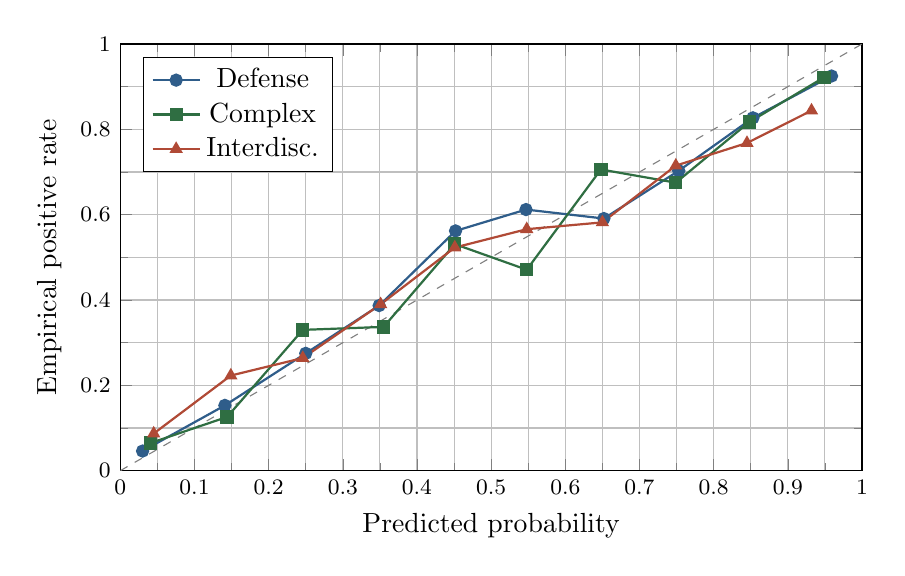
\begin{tikzpicture}
\begin{axis}[width=11cm, height=7cm, xlabel={Predicted probability}, ylabel={Empirical positive rate},
  xmin=0, xmax=1, ymin=0, ymax=1, legend pos=north west, grid=both, minor tick num=1, tick label style={font=\footnotesize}]
\addplot[dashed, gray, forget plot] coordinates {(0,0)(1,1)};
\addplot[accent, mark=*, thick] coordinates {(0.03,0.046)(0.141,0.153)(0.25,0.275)(0.349,0.387)(0.452,0.562)(0.547,0.612)(0.652,0.591)(0.753,0.703)(0.853,0.827)(0.959,0.925)};
\addlegendentry{Defense}
\addplot[good, mark=square*, thick] coordinates {(0.041,0.065)(0.144,0.126)(0.246,0.33)(0.355,0.337)(0.451,0.531)(0.548,0.471)(0.648,0.706)(0.749,0.675)(0.848,0.817)(0.949,0.922)};
\addlegendentry{Complex}
\addplot[clay, mark=triangle*, thick] coordinates {(0.045,0.087)(0.149,0.223)(0.246,0.264)(0.351,0.39)(0.451,0.523)(0.548,0.566)(0.65,0.582)(0.749,0.715)(0.845,0.768)(0.932,0.844)};
\addlegendentry{Interdisc.}
\end{axis}
\end{tikzpicture}
\end{center}

\begin{center}
\begin{tabular}{@{}lccc@{}}
\toprule
\textbf{Model} & \textbf{AUROC} & \textbf{Brier} & \textbf{ECE} \\
\midrule
Defense & 0.897 & 0.129 & 3.4\% \\
Complex-Invention & 0.874 & 0.144 & 4.1\% \\
Interdisciplinary & 0.754 & 0.203 & 5.0\% \\
\bottomrule
\end{tabular}
\end{center}

\noindent Expected calibration error is $\leq 5\%$ for all three (best for Defense),
so a reported score reads as a genuine probability, and the model expresses honest
uncertainty rather than overconfident automation. \textbf{Caveat:} these are
calibrated to the balanced training distribution; scoring the rare-positive
real-world population needs a base-rate (prior) correction --- a one-line post-hoc
adjustment.

\section{Timeline status (June 2025 -- January 2027)}
\begin{center}
\begin{tabular}{@{}p{3.4cm}p{8.5cm}c@{}}
\toprule
\textbf{Semester} & \textbf{Milestone vs.\ delivered} & \textbf{Status} \\
\midrule
Jun--Dec 2025 & Score Duke output (base scores exist; new-model Duke batch pending); \emph{initiate} specialized model training $\rightarrow$ \textbf{fully trained + deployed}; GPT agent prototype $\rightarrow$ \textbf{live agent}. & \stDone \\
Jan--Jun 2026 & Beta agent interface $\rightarrow$ \textbf{done}; specialized scores + validation $\rightarrow$ \textbf{validated on held-out}; Duke output scored on Scientifiq.AI. & \stDone \\
Jul--Dec 2026 & Improved agent $\rightarrow$ early; finalize toolkit \& dashboard $\rightarrow$ \textbf{Agent + Batch + Explorer + six-dim fingerprint}; white paper + open-source $\rightarrow$ pending. & \stSub \\
\bottomrule
\end{tabular}
\end{center}
Net: the modeling and agent milestones are complete ahead of schedule; the
remaining timeline items are dissemination (white paper, open-source) and the
Duke-wide scoring pass.

\section{How to reach everything}\label{sec:access}
Keys / superadmin access are shared separately; the paths are stable.
\begin{itemize}[leftmargin=1.4em, itemsep=1pt]
  \item \textbf{Scoring API (all models):} \texttt{POST} to
  \url{https://sciscore-1029497676656.us-central1.run.app/score} with
  \texttt{Authorization: Bearer <SCISCORE\_API\_KEY>} and body
  \texttt{\{"task":"defense\_impact"|"complex\_invention"|"interdisciplinary","text":"..."\}}
  (\texttt{GET /tasks} lists them; a \texttt{texts:[...]} array scores in batch).
  \item \textbf{Impact fingerprint (all six potentials):} the \emph{Score My
  Invention} module --- paste an abstract, get commercial/scientific/social plus
  complex-invention and interdisciplinary (and defense, for directors).
  \item \textbf{Defense Impact:} module at \url{https://superadditive.app/start/defense-impact};
  public API \texttt{POST /api/v1/defense-impact} (bearer key). Director-gated.
  \item \textbf{Research Agent:} \url{https://superadditive.app/agent}.
  \item \textbf{ExplainAI:} the \emph{ExplainAI} module --- paste an abstract, get plain-language framings for four audiences.
  \item \textbf{Ecosystem Explorer:} inside the Domain Brief module.
  \item \textbf{Batch scorer:} \url{https://superadditive.app/batch} (directors).
  \item \textbf{Lab hub:} \url{https://superadditive.app/duke-isp}.
\end{itemize}

\section{Reproducibility}\label{sec:repro}
In the repository under \texttt{ml/}:
\texttt{sciscore/} (train + infer + serve), \texttt{sql/} (BigQuery labeling
queries for all three datasets), \texttt{tasks/} (one YAML per model),
\texttt{models/} (trained heads, baked into the Cloud Run image), and
\texttt{notebooks/} (a Colab training notebook, no local setup). Rebuilding a model:
run its \texttt{sql} query to a CSV, then
\texttt{sciscore train --task ml/tasks/<name>.yaml --data <name>.csv --out models/<name>},
then redeploy.

\section*{What remains}
One formality: \textbf{tag the new models into the existing public GitHub/Zenodo
release} and fold the results into the white paper. All seven deliverables are
otherwise complete or delivered.

\end{document}
